\documentclass[12pt]{article}

\usepackage{amsmath, color}
\usepackage{mdwmath}
\usepackage{amssymb, epsf, epsfig, textcomp}
\renewcommand{\baselinestretch}{1.3}
\usepackage{a4wide}
\newcommand{\argmin}{\mathop{\mathrm{argmin}}}
\usepackage{caption}
\usepackage{subcaption}
\usepackage{mathtools}

\usepackage{amsmath}	% Align equations: align, gather
\usepackage{amssymb}	% Math symbols: http://milde.users.sourceforge.net/LUCR/Math/mathpackages/amssymb-symbols.pdf
\newcommand\numberthis{\addtocounter{equation}{1}\tag{\theequation}}	% Number any line of an equation, can be used at end of align*

\usepackage{enumitem}	% Custom enumeration: [label=(\arabic*)], [label=(\roman*)]
\usepackage{moreenum}	% Custom enumeration: [label=(\greek*)]

\usepackage{listings}
\lstdefinestyle{myCustomMatlabStyle}{
	basicstyle=\ttfamily\footnotesize,
	breaklines=true,
	language=Matlab,
	numbers=left,
	stepnumber=1,
	numbersep=10pt,
	tabsize=4,
	showspaces=false,
	showstringspaces=false
}
\begin{document}
	\noindent\rule{\textwidth}{2pt}
	\begin{center}
		{\bf Technical University of Crete}\\
		{\bf School of Electrical and Computer Engineering} \\
		Course: {\bf Advanced Topics in Convex Optimization} \\
		Instructor: Athanasios P. Liavas \\
	\end{center}
	{\bf Student: }Alevrakis Dimitrios 2017030001\\
	\rule{\textwidth}{.5pt}
	\vskip .1cm
	\noindent

	\begin{enumerate}
		\item[\bf Part A]
			\begin{enumerate}
				\item[1]
				Computation of the projection onto the unit simplex.\\
				
				The unit Simplex: $\Delta_n=\{{\bf x}\in\mathbb{R}^n : {\bf x} \geq {\bf 0},{\bf e}^T{\bf x}=1\}$.\\
				
				There for the problem can be written as:\\
				\begin{align*}
					&\text{min } f({\bf x})=\frac{1}{2}||{\bf{x_0}-{\bf x}}||^2_2\\
					&\begin{array}{cc}
						\text {s.t. }&{\bf e}^T{\bf x} = 1\\
						& {\bf x}\geq {\bf 0}
					\end{array}
				\end{align*}
			
				\item[3] Let ${\bf c\in \mathbb{R}^n}$ and $\Delta_n=\{{\bf x}\in\mathbb{R}^n : {\bf x} \geq {\bf 0},{\bf e}^T{\bf x}=1\}$.\\
				The problem:
				\begin{align*}
					\begin{array}{c}
						\text{min }_{{\bf x\in \Delta_n}} f({\bf x})={\bf c}^T{\bf x}
					\end{array}
				\end{align*}
				Which can be written as:
				\begin{align*}
					&\text{min }_{{\bf x}\in \mathbb{R}^n} f({\bf x})={\bf c}^T{\bf x}\\
					&\begin{array}{cc}
						\text {s.t.}&h({\bf x})={\bf e}^T{\bf x} -1 = 0\\
						& f_i({\bf x})=-x_i\leq {\bf 0},\ i=1,...n
					\end{array}
				\end{align*}
			
				The KKT for this problem are:
				\begin{align*}
					&\nabla f({\bf x}) + \sum_i^n u_i\nabla f_i({\bf x}) + {\bf e}v = 0 \Rightarrow{\bf c} + {\bf u} + {\bf e}v = 0 \numberthis\\
					&u_i\geq0,\ i=1,...,n \numberthis\\
					&u_ix_i= 0,\ i=1,...n \numberthis\\
					&v\in\mathbb{R}
				\end{align*}
			
				\begin{figure}[h]
					\caption{Examples ${\bf c}^T{\bf x}$ Level Sets and the minimum on $\Delta_2$}
					\centering
					\begin{subfigure}[b]{0.4\textwidth}
						\centering
						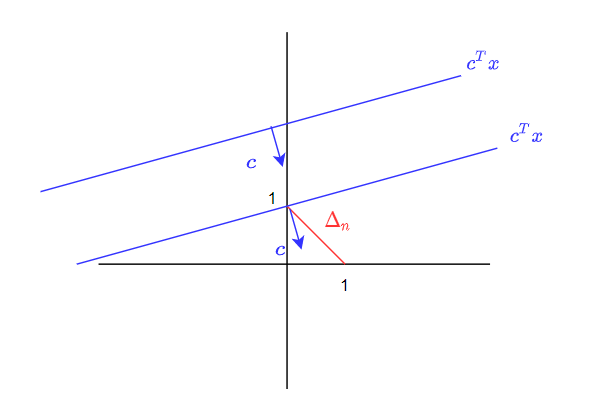
\includegraphics[width=\textwidth]{P2-fig0.png}
					\end{subfigure}
					\begin{subfigure}[b]{0.4\textwidth}
						\centering
						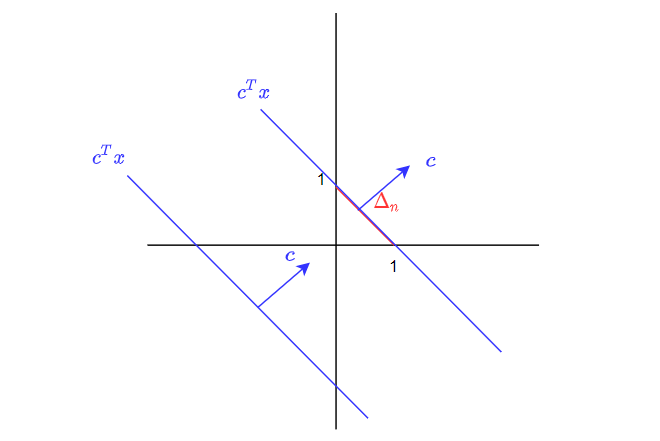
\includegraphics[width=\textwidth]{P2-fig1.png}
					\end{subfigure}
				\end{figure}
				
				As observed on the above examples we claim that a minimum ${\bf x^*}$ always has an element $x^*_k = 1,\ k=1,...,n$\\
				
				Therefore $x^*_k=1$, using (3): \\
				\begin{align*}
					&u_kx^*_k=0 \overset{x^*_k=1}{\Rightarrow}u_k=0\\
					&(1)\Rightarrow c_k + v=0 \iff v=-c_k\numberthis
				\end{align*}
				
				Replacing (4) in (1) an solving for ${\bf u}$ we get:
				\begin{align*}
					{\bf u} = {\bf e}c_k-{\bf c} \Rightarrow u_i = c_k-c_i,\ i=1,...,n\numberthis
				\end{align*}
			
				From (2) and (5) we get that: $\displaystyle c_i\geq c_k$.
				
				Therefore we can say that the solution ${\bf x^*}$ is 1 at $k = min_i{\bf c}$ and 0 at the other indices
			\end{enumerate}
	\end{enumerate}
	
	
	
\end{document}
